%!TEX root = Thesis.tex
\chapter{Concept}
     The chapter describes a concept of a generic frontend for exploring sensor data, 
     that in the same time controlled and provisioned by end users request. 
     The concept is developed based on the analysis of the current
     state of the platform, the defined requirements to the third-party services and applications
     (section X.X) and knowledges gained from the studied related works (chapter 3).

\begin{itemize}
     \item  Concept for a generic information and sensor service portal
      \item Development of the portal and associated dependency tools
\end{itemize}

\section{Requirements}

\subsection{Functional Requirements}

\subsection{Non-functional Requirements}

\begin{figure}[!ht]
\centering
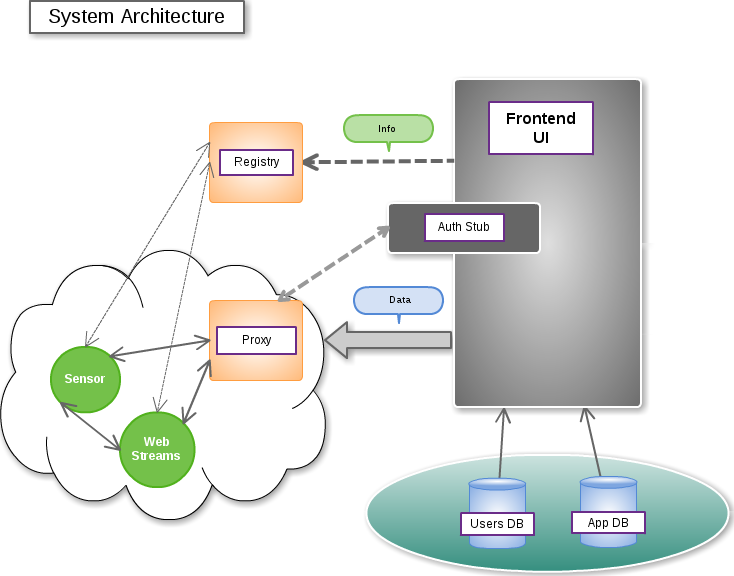
\includegraphics[scale=0.5]{images/Structure.png}   % path to image file in PNG
\caption[System Architecture]{System Architecture}
\label{img:structure}                           % label for references
\end{figure}
%\footnotetext{Image taken from \url{blog.csdn.net/cain/article/details/6617173}}

\section{Architecture}
\section{Frontend}

\section{Summary}
In this master thesis, a first web-based prototype (portal) for such services is to be
created. Along with it, a light-weight scenario service registry will be needed. Users
should be able to explore not just services, but also the information provided by
them, and eventually be led to advanced usage patterns such as the development
of third-party applications to access the information data and real-time streams.